% DO NOT REMOVE
% 43423322556654566777777364443365

\documentclass[12pt]{article}

% PACKAGES
\usepackage[english]{babel}
\usepackage[utf8]{inputenc}
\usepackage{graphicx}
\usepackage{xcolor}
\usepackage{listings}
\usepackage{wrapfig}
\usepackage[T1]{fontenc}
\usepackage[scaled=0.85]{beramono} % For bold teletype font

% CONFIGURATIONS
\graphicspath{ {./images/} }

\definecolor{codegreen}{rgb}{0,0.6,0}
\definecolor{codegray}{rgb}{0.5,0.5,0.5}
\definecolor{codepurple}{rgb}{0.58,0,0.82}
\definecolor{backcolour}{rgb}{0.95,0.95,0.92}
\lstdefinestyle{cstyle}{
    backgroundcolor=\color{backcolour},
    commentstyle=\color{codegreen},
    keywordstyle=\color{blue},
    numberstyle=\tiny\color{codegray},
    stringstyle=\color{codepurple},
    basicstyle=\ttfamily\scriptsize,
    breakatwhitespace=false,         
    breaklines=true,
    captionpos=b,
    keepspaces=true,
    numbers=left,
    numbersep=5pt,
    showspaces=false,
    showstringspaces=false,
    showtabs=false,
    tabsize=2
}
\lstset{style=cstyle}

\newcommand{\code}[1]{\texttt{#1}}
\newcommand{\name}{\textsc{Connect Four}}

% DOCUMENT BODY CONTENT
\begin{document}

% Title Page
\begin{titlepage}
	\centering
        {\scshape\Large Artificial Intelligence Final Project\par}
        \vspace{0.5cm}
        {\scshape\small COMP.4200 Artificial Intelligence, Fall 2022 \par}
        \vspace{0.5cm}
	{\scshape Miner School of Computer \& Information Sciences\par
        University of Massachusetts Lowell\par}

	\vspace{1.5cm}
	{\huge\bfseries Solving Connect Four with AI\par}
	\vspace{0.5cm}
	{\large\bfseries Applying Machine Learning to Complex Problems\par}
	\vspace{1.5cm}
	{\Large Sepehr Madani, Jacob Veber\par}
	\vfill
	{\large Fall 2022\par} % Bottom of the page
\end{titlepage}

\begin{abstract}
Examining the application of artificial intelligence techniques used to solve \name\ gives us an insightful and practical study of the AI theories in a real-world application. In this paper, we observe and examine the advantages that different optimization algorithms offer, namely, \texttt{MinMax} and \texttt{Alpha-Beta} pruning, which furthers our understanding of how we may apply AI to other fields of research.\par
There are also strategies specific to ensuring a victory in \name\ that reveal how a problem can be broken apart and digested, giving a foundation to build a solution from.\par
\vfill
\noindent\textbf{Keywords:} machine learning; game theory; artificial intelligence, alpha-beta pruning

\end{abstract}


\section{Context and Motivation}
Studying the field of Artificial Intelligence (AI) has offered an abundance of new insights into how we may approach different computational problems.  One particular branch of mathematics, game theory, has exploded since its merger with AI research.  By researching game theory, scientists aim to develop an understanding of the causal relationships held between decision-making and their outcomes.  

Such examinations can reveal findings not only in applied mathematics and computer science, but across other fields as well, such as in economics, biology, and the social sciences.  These fields have been notoriously challenging to model because of how many variables one must consider when predicting an outcome.  Examining environments with fewer variables and less complicated rule-sets allows us to apply findings to more complex systems. One way mathematicians have done this is by solving games of increasing complexity, in other words, making every outcome exactly predictable given a position and assuming perfect play.  Games like \textit{nim} and \textit{Tic-Tac-Toe} fall into this category, while Chess and Go do not yet have a guaranteed winning or drawing strategy (although they are theoretically solvable)\footnote{There exist AIs that play \textit{Chess} and \textit{Go} at an exceptional level, exceeding that of their respective Grand Champions.}\cite{kdnuggets}.

In this paper, we examine the game of \textbf{\textsc{Connect Four}} (also known as \textit{Captain's Mistress}, \textit{Four in a row}, among others).

\subsection{Game Rules}
\name\ is a two-player board game with perfect information for both sides played on a vertical board consisting of six rows and seven columns. We can classify \name\ as an adversarial, zero-sum game.

Players each have 21 chips. First player has yellow, and second player has red chips.
They make moves in turns, by dropping their chips into the board from the top, falling to the lowest unoccupied space in the column. The first player to obtain four \textit{connected} chips horizontally, vertically, or diagonally, wins (essentially, making four in a row; hence the name). If neither of the players obtain a connected four set of chips and the board is filled (by which time neither have any more chips left), the game is a draw.
An example of the winning configuration for yellow is shown below.

\begin{figure}[h]
\centering
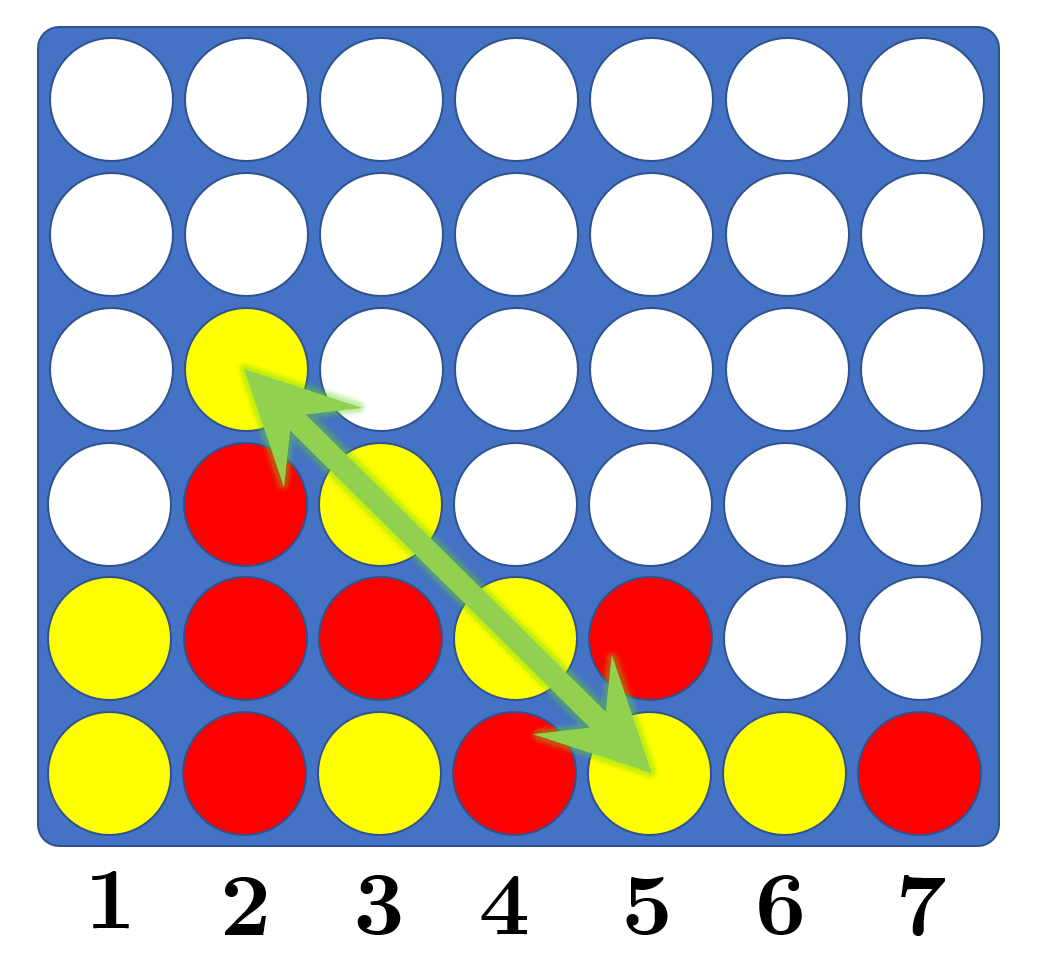
\includegraphics[width=5cm]{position-1.png}
\label{fig:sampleposition}
\caption{A winning position for yellow, achieving a diagonal four chips in a row.}
\end{figure}

\subsection{Complexity}
In terms of complexity, \name\ falls somewhere  between Tic-Tac-Toe and Chess, having an astounding 4,513,985,219,092 possible game configurations. \cite{trompnumber}
With Tic-Tac-Toe having already been trivially solved \cite{tictactoe} and chess being unsolved \cite{kumar2021can}, \name\ is a perfect candidate to examine for an applied study of Artificial Intelligence.

\section{Winning Strategy}
\subsection{History}
\name\ is shown to be a first-player-win; in other words, with perfect play, the first player can always force a win.\cite{allen_2010}

In 1988, two people solved \name\ through independent studies; James Dow Allen \cite{allen_2010}, and Victor Allis \cite{allis1988knowledge}.
Computers at that time were not yet powerful enough to solve the game through sheer brute force by checking every possible move, so the two researchers detailed a series of different strategies to ensure the best chance at victory.
Since then, AI methods using different optimization algorithms have emerged to solve the game with varying degrees of success and efficiency.
A study of the techniques used to solve \name\ can prove useful for gaining a better insight into AI in game theory as well as other fields.

Allis' analysis consists of discussing the ineffectiveness of a brute-force approach (citing the weakness of computational power at the time, as mentioned before) and proposing a \textit{knowledge-based} approach. He formally outlines 9 rules named \texttt{Claimeven}, \texttt{Baneinverse}, \texttt{Vertical}, \texttt{Aftereven}, \texttt{Lowinverse}, \texttt{Highinverse}, \texttt{Baseclaim}, \texttt{Before}, \texttt{Specialbefore}, the first four outlining the most elementary rules that any experienced \name\ player will observe. The author implements all said rules in the solver program \texttt{VICTOR}, however, a detailed discussion of this approach is beyond the scope of this paper. Therefore, in the interest of time, we will leave it to the reader \cite{allis1988knowledge}.

Lastly, it is worth noting that \name\ has since been solved with brute-force by creating an 8-ply database. The reader is free to explore the findings on John Tromp's Connect Four Playground \cite{trompplayground}.

\subsection{Our Approach for the Strategy}

\subsubsection{Notation}
For the discussion of the strategy, we first denote the first player playing yellow chips as $A$ and the second player playing red chips as $B$.
We also define a numerical coordinate system on the board, assigning $1$ through $7$ to their respective \textbf{columns} from left to right. Every position in the board is referenced to as a \textbf{square}.

\begin{wrapfigure}{r}{0.25\textwidth}
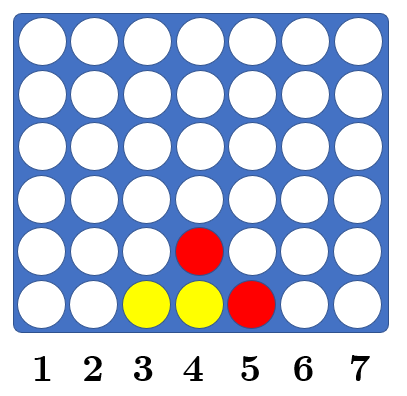
\includegraphics[width=1\linewidth]{position-2.png} 
\caption{Position described by $4435$.}
\label{fig:wrapfig}
\end{wrapfigure}

We also describe any game position after $n$ moves as a sequence of digits, $a_1a_2a_3\cdots a_n$, where $a_i \in \{1, 2, \cdots, 7\}$ describing the played column.  For instance, the position $4435$ describes the board shown to the right.

One can also verify that the positions in figure \ref{fig:sampleposition} can be described as $12345765431243322$, or $34125547624332152$. Note that we do not care that a position cannot be described uniquely, since our purpose is to easily feed any position to the program to begin the search algorithm from.

\section{Applying Artificial Intelligence Techniques}

\subsection{Heuristic Score Function}
For evaluating each position for whether $A$ or $B$ can win, we set a scoring system as follows.

For any non final position reflecting the outcome of the game for the player to play, considering that both players play perfectly and try to win as soon as possible or lose as late as possible. A position has:
\begin{itemize}
    \item a positive score if the current player can win. 1 if he wins with her last chip, 2 if she wins with her second last chip, and so on.
    \item a null score if the game will end by a draw.
    \item a negative score if the current player would lose regardless of what she plays. -1 if her opponent wins with his last chip, -2 if her opponent wins with his second last chip, and so on.
\end{itemize}

Positive (winning) score can be computed as 22 minus number of chip played by the winner at the end of the game. Negative (losing) score can be computed as number of chip played by the winner at the end of the game minus 22. Note that 22 is one plus the number of initial chips with each player.

% One can notice that after playing the best move, the score of one's opponent is the opposite of one's score.

For instance, position "4455" has a score of 18, because the $A$ can win in two moves with his 4th chip, yielding $22 - 4 = 18$.

\begin{figure}[h]
\centering
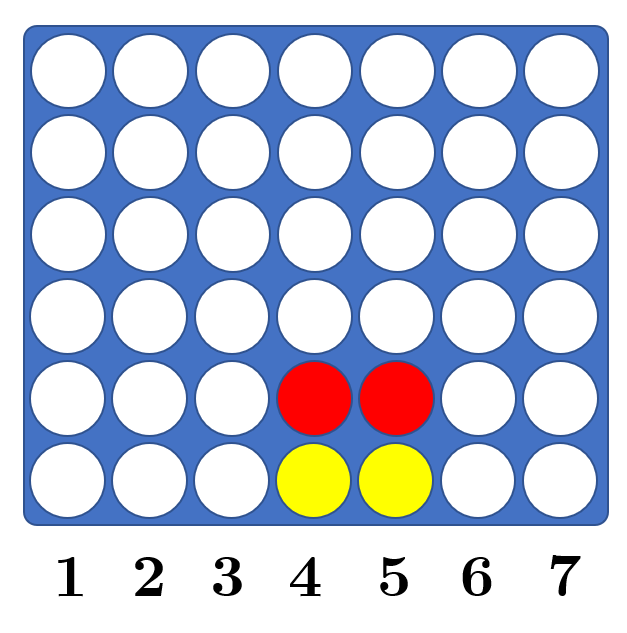
\includegraphics[width=3.5cm]{position-3.png}
\caption{A winning position for $A$, using her 4th chip.}
\end{figure}

% Fundamentally, these definitions serve to assign every playable action a positive or negative weight, which will help us to design our approach to a solution. 

\subsection{The \texttt{MinMax} Algorithm}
The most simple technique for solving \name\ is the \texttt{MinMax} algorithm. In this technique, we are finding the shortest path possible in the game's decision tree where each node is a position, and each move is an edge connecting two different nodes.

As previously mentioned, each possible move is given a score that describes whether the new position after that move gives the player a better or worse chance at victory, assuming best play by both players. In essense, \texttt{MinMax} aims to \textit{min}imize the \textit{max}imum loss that a player would sustain after each move.

% These values are evaluated assuming the worst-case scenario, predicting that the opponent will make the decision that puts them in the best position. This observation arms us with the idea to search the game tree of all possible outcomes to find the winning path. The player is then incentivized to make the move that maximizes the value of their position and minimizes the value of their opponent's.

This study uses a variant of the \texttt{MinMax} algorithm called \texttt{\textbf{NegaMax}} that condenses the opponent and player scores into a single value.  We are leveraging that the opponent's positional value is always the additive inverse (negative) of the player's value (in other words, $S_A + S_B = 0$).

While \texttt{MinMax} provides the foundation for how the computer makes its moves, it is still a rather primitive approach to finding a solution.  On its own, the algorithm is highly inefficient and will explore unnecessary pathways, such as those with a lower score than an already discovered node.  In practice this leads to a disappointing performance and memory usage.

This is observed in Pascal Pons' study, in which test sets of 1,000 different board positions were separated into 6 different groups depending on the number of moves that had been played, and how many were left to play to win. All test sets with less than 29 moves played (which is considered to be well into the endgame) were unable to be calculated within 24 hours of the \texttt{MinMax} algorithm being run \cite{solvingconnect}.

To make improvements to the time and unnecessary computing, we turn to Alpha-Beta Pruning for optimization.

\subsection{Alpha-Beta Pruning}
With Alpha—Beta Pruning technique, we "prune" the decision tree by limiting the scores examined by the program to the bound $[\alpha, \beta]$. This reduces the nodes explored in the search tree; that is, if we, for instance, have explored a move with a score of 10, there is no need to explore nodes with scores lower than 10 in the tree. Furthermore, we tighten $[\alpha, \beta]$ as we continue the search, beginning with $[\alpha, \beta] = [-\infty, \infty]$.

Another benefit of the Alpha-Beta approach is that we can easily implement a weak solver that only tells us the win/draw/loss outcome of a position by calling the evaluation function a node with the $[-1,1]$ score window.
% This allows for the scope to be adjusted so that long run times can be avoided.

With the addition of this technique, the number of positions that are searched is greatly reduced.  This allows for the test sets of 1,000 cases, each with more than 14 moves already played to be solved in under 24 hours \cite{solvingconnect}.  This is a direct improvement from strictly using the \texttt{MinMax} function, solving the set with over 28 moves played faster, and finishing calculation on sets that took over 24 hours without Alpha-Beta Pruning.

A documented implementation of the \texttt{NegaMax} function with \textbf{Alpha-Beta Pruning} is available on page 7.

\section{Concluding Thoughts}
As we saw, even a unconvoluted technique such as the alpha-beta pruning can be employed to solve a game as sophisticated as \name. Such a program can even be scaled enough to be employed as a viable computer bot for children to practice against. Furthermore, alpha-beta pruning provides the basis for more advanved techniques such as transposition tables and iterative deepening which have higher performances. However, we leave for future studies. For a more detailed reference, see \cite{allis1988knowledge}, \cite{solvingconnect}, and \cite{trompplayground}.

\newpage
\section*{Appendix A. Reference Code}
\lstinputlisting[language=C++]{./code/alphabeta.cpp}

\newpage
\bibliographystyle{abbrv}
\bibliography{bib}

\end{document}